\documentclass[tikz,border=8pt]{standalone}
\usepackage{amsmath}\usepackage{pgfplots}\pgfplotsset{compat=1.18}\usetikzlibrary{arrows.meta}
\definecolor{ink}{HTML}{334155}\definecolor{blue}{HTML}{6366F1}\definecolor{green}{HTML}{059669}\definecolor{orange}{HTML}{EA580C}
\begin{document}
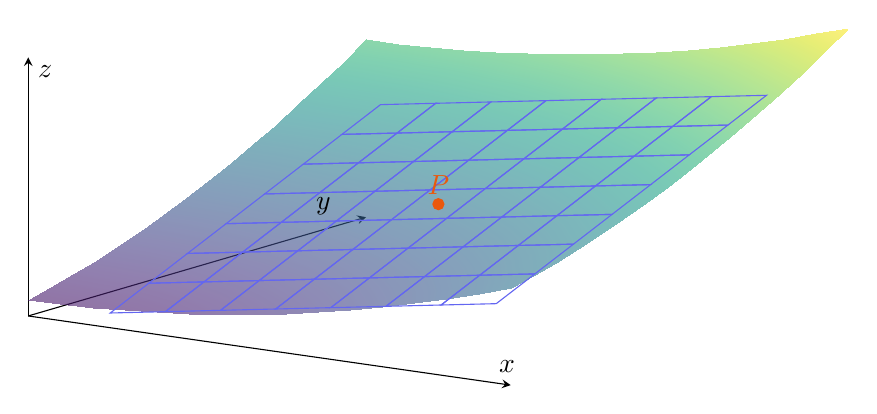
\begin{tikzpicture}\begin{axis}[width=12cm,height=7cm,view={35}{25},axis lines=center,xlabel=$x$,ylabel=$y$,zlabel=$z$,ticks=none,xmin=0,xmax=2,ymin=1,ymax=3]
\addplot3[surf,opacity=.6,shader=interp,domain=0:2,y domain=1:3,samples=16,colormap/viridis]{x^2+y^2};
\addplot3[mesh,blue,domain=.2:1.8,y domain=1.2:2.8,samples=8]{2*x+4*y-5};
\addplot3[only marks,mark=*,mark size=2pt,orange]coordinates{(1,2,5)}node[above]{$P$};\end{axis}\end{tikzpicture}
\end{document}
